\section{Gradient Descent}

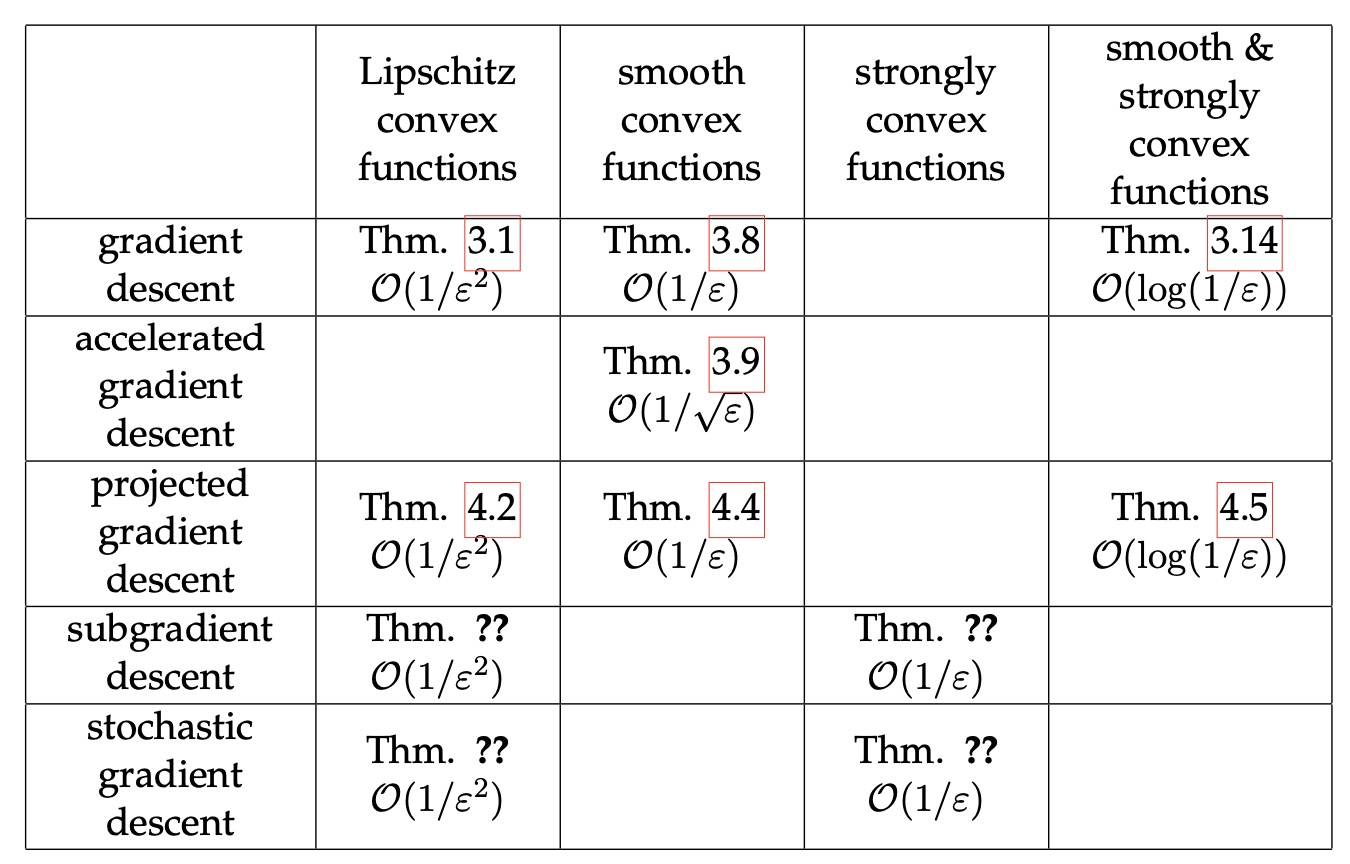
\includegraphics[width=\linewidth]{imgs/GD.jpg}

Define $g_t = \nabla f(x_t)$. The gradient descent is $x_{t+1} = x_t - \gamma g_t$, where $\gamma$ is the step size. We assume $f$ is differentiable anywhere.

\textbf{Definitions}:
\begin{enumerate}
    \item A convex differentiable function $f$ is $L$-smooth if $f(y) \le f(x) + \nabla f(x)^\top (y-x) + \frac{L}{2}\|x-y\|^2$ for any $x, y$.
    \item A function is $\mu$-strongly convex if $f(y) \ge f(x) + \nabla f(x)^\top (y-x) + \frac{\mu}{2}\|x-y\|^2$ for any $x, y$.
\end{enumerate}

\textbf{Properties}:
\begin{enumerate}
    \item \textbf{Characterization of $L$-smoothness (equivalent)}: (3.3) $\frac{L}{2}x^\top x - f(x)$ is convex; (3.5) $\|\nabla f(x) - \nabla f(y)\| \le L \|x-y\|$ for any $x,y$;
    \item \textbf{Operations that perserve smoothness} (3.6): (i) Assume $f_i$ are $L_i$-smooth and $\lambda_i >0$, then $f:= \sum_{i} \lambda_i f_i$ is $\sum_i \lambda_i L_i$-smooth. Proof by (3.3). (ii) Assume $f$ is $L$-smooth and $g(x) = Ax+b$, then $f\circ g$ is $L\|A\|^2$-smooth.
    \item \textbf{Characterization of $\mu$-strongly convexity (equivalent)}: (3.11) $f(x) - \frac{\mu}{2}x^\top x$ is convex.
    \item \textbf{Bound of first-order changes}: Let $f$ be convex and $x^*$ be the global minimum, i.e. $\nabla f(x^*) = 0$. If $f$ is $\mu$-strongly convex, then $\nabla f(x)^\top (x - x^*) \ge \mu \|x-x^*\|^2$. If $f$ is $L$-smooth, then $\nabla f(x)^\top (x - x^*) \le L \|x-x^*\|^2$. Proof: write definition separately for $x^*$ on $x_t$ and $x_t$ on $x^*$, then add the two inequalities together.
\end{enumerate}

Analysis based on the first-order characterization:
\begin{enumerate}
    \item Vanilla analysis (no further assumption): by first-order characterization, we can bound $f(x_t)-f(x^*) \le g_t^\top (x_t - x^*)$. The algorithm says $g_t = (x_t - x_{t+1}) / \gamma$, thus $g_t^\top (x_t - x^*) = \frac{1}{\gamma} (x_t - x_{t+1})^\top (x_t - x^*)$. Since $2a^\top b = a^\top a + b^\top b - (a-b)^\top (a-b)$, we have $2(x_t - x_{t+1})^\top (x_t - x^*) = \|x_t - x_{t+1}\|^2 + \|x_t - x^*\|^2 - \|x_{t+1} -x^*\|^2$. Therefore, $\sum_{t=0}^{T-1}(f(x_t)-f(x^*)) \le \sum_{t=0}^{T-1} g_t^\top (x_t - x^*) \le \frac{\gamma}{2}\sum_{t=0}^{T-1}\|g_t\|^2 + \frac{1}{2\gamma} \|x_0-x^*\|^2$.  The problem is to bound the squared norm of gradients.
    \item Lipschitz convex functions: bounded gradients $\|\nabla f(x)\| \le B$ for any $x$. (3.1) Assume $\|x_0 - x^*\| \le R$.  Then the result of vanilla analysis says $\sum_{t=0}^{T-1}(f(x_t)-f(x^*)) \le \frac{\gamma}{2}B^2 T + \frac{1}{2\gamma}R^2$. Choose $\gamma=\frac{R}{B\sqrt{T}}$ yields $\frac{1}{T}\sum_{t=0}^{T-1}(f(x_t)-f(x^*)) \le \frac{RB}{\sqrt{T}}$. This means we need $T\ge R^2B^2/\epsilon^2$ to achieve $\min_t (f(x_t)-f(x^*)) \le \epsilon$. 
\end{enumerate}

Analysis based on control over the quadratic term:
\begin{enumerate}
    \item $L$-smooth functions (not requiring convexity): (3.7) with $\gamma:=1/L$, we have $f(x_{t+1}) \le f(x_t) - \frac{1}{2L}\|\nabla f(x_t)\|^2$. Proof: use smoothness definition and plug in $x_{t+1}-x_t = -\frac{1}{L}\nabla f(x_t)$.
    \item Convex $L$-smooth functions: (3.8) with $\gamma:=1/L$, we have $f(x_T) - f(x^*) \le \frac{L}{2T}\|x_0 - x^*\|^2$. This means we only need $T \ge \frac{R^2 L}{2\epsilon}$ to achieve error at most $\epsilon$. Proof: by (3.7), $\frac{1}{2L}\sum_{t=0}^{T-1} \|\nabla f(x_t)\|^2 \le f(x_0) - f(x^*)$. Plugging into vanilla analysis, we have $\sum_{t=1}^T (f(x_t) - f(x^*)) \le \frac{L}{2}\|x_0 - x^*\|^2$. By (3.7), $f(x_t) - f(x^*)$ is monotonically decreasing, thus $f(x_T) - f(x^*) \le \frac{L}{2T}\|x_0 - x^*\|^2$. 
    \item $\mu$-strongly convex and $L$-smooth functions: (3.14) GD with $\gamma = 1/L$ yields $\|x_{t+1}-x^*\|^2 \le (1-\frac{\mu}{L})\|x_t - x^*\|^2$ and $f(x_T) - f(x^*) \le \frac{L}{2}(1-\frac{\mu}{L})^T \|x_0 -x^*\|^2$. This means we need $T \ge \frac{L}{\mu}\log\left(\frac{R^2 L}{2\epsilon}\right)$ to achieve error at most $\epsilon$. Proof: (i) replacing the first-order characterization in the vanilla analysis by the condition of $\mu$-strongly convexity, we get $\|x_{t+1}-x^*\|^2 \le 2\gamma \left(f(x^*) - f(x_t)\right) + \gamma^2 \|\nabla f(x_t)\|^2 + (1-\mu\gamma)\|x_t - x^*\|^2$. By sufficient decrease of $L$-smooth functions, we have $f(x^*) - f(x_t) \le f(x_{t+1}) - f(x_t) \le -\frac{1}{2L}\|\nabla f(x_t)\|^2$. Combining these two gives the first result. (ii) By smoothness, $f(x_T) - f(x^*) \le \frac{L}{2}\|x_T - x^*\|^2 \le \frac{L}{2}(1-\frac{\mu}{L})^T \|x_0 -x^*\|^2$. 
\end{enumerate}

\textbf{Optimizing without knowing $L$ or $B$}: for $L$-smooth convex functions, we do not need to know $L$ to ensure $O(\frac{R^2 L}{\epsilon})$ steps. The idea is to guess $L$ and refine it gradually. The first guess is $L_0 := \frac{2\epsilon}{R^2}$. For each guess, we check if the sufficient decrease (3.7) holds. If (3.7) holds in the whole process $T = \frac{R^2 L_i}{2\epsilon}$, then $L_i$ is a successful guess, and we finish. If the guess is incorrect, we double $L_{i+1} = 2L_i$ and repeat. The final guess cannot exceed two times the correct value, and the number of iterations is bounded by $\sum_i 2^i$ until the last term exceeds the true $L$. This means the total number of iterations is bounded by two times the last iteration time, which is still $O(\frac{R^2 L}{\epsilon})$. A similar approach can be taken for Lipschitz convex functions to optimize without knowing $B$.

\textbf{Accelerated Gradient Descent}

The AGD is to do $y_{t+1}= x_t - \frac{1}{L}\nabla f(x_t)$, $z_{t+1} = z_t - \frac{t+1}{2L}\nabla f(x_t)$ and $x_{t+1} = \frac{t+1}{t+3} y_{t+1} + \frac{2}{t+3}z_{t+1}$. Initialized with $y_0=z_0 = x_0$.

(Thm 3.9) For $L$-smooth convex functions, AGD yields $f(y_T) - f(x^*) \le \frac{2L\|z_0 - x^*\|^2}{T(T+1)}$.